\begin{slide}{Project Context and Objectives}
	{\large \textbf{Idea:} Use reaction-diffusion to build explicit spatial dependence.}
	\begin{columns}[T]
		\begin{column}{.6\textwidth}
			\vspace{2cm}
			\begin{itemize}
				\item The data clearly shows a diffusive pattern
				\item Spatial dependence can approximate demographic differences
				\item Spatially dependent data exists for many scales and regions
			\end{itemize}
		\end{column}
		\begin{column}{.4\textwidth}
			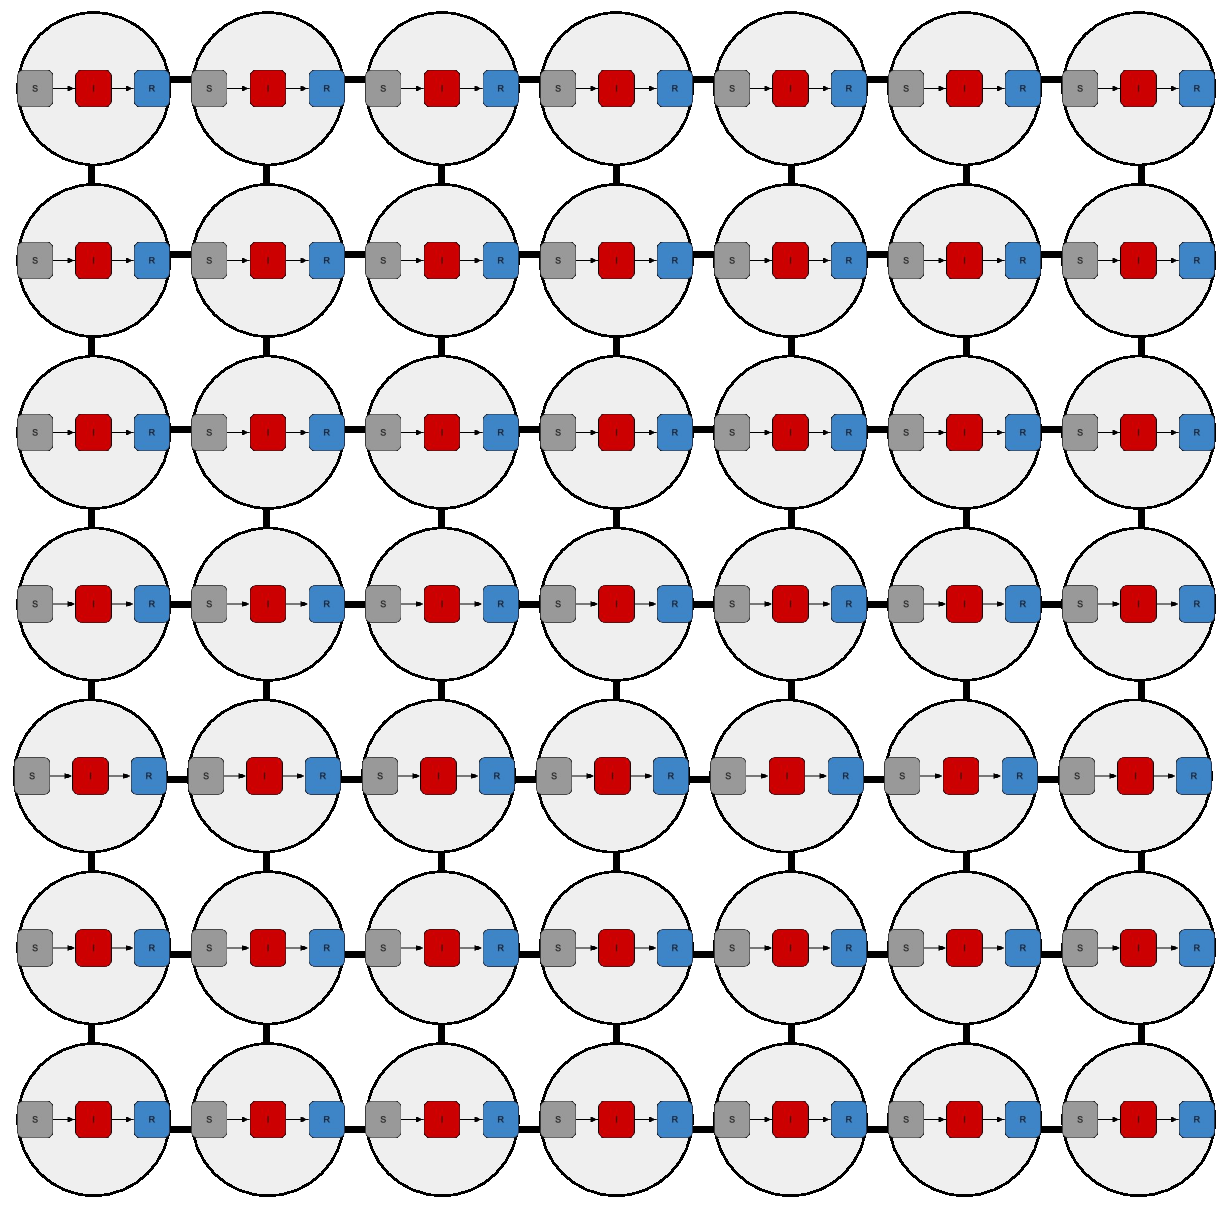
\includegraphics[height=6cm]{images/spatial-grid}
		\end{column}
	\end{columns}
\end{slide}